% !TeX root = ../main.tex

\section*{Markov Random Fields (MRF)}

Example use cases are denoiseing, segmentation or stero matching. \footnote{Geman / Geman introduced MRF to image processing (1985)} Consider the pixel gird as a lattice of random variables. More specifically let us asume, that the image $F$ is given by the random matrix $[f_{i,j}]$.

Assumption: limited statisical depenency (between the pixels)

\begin{equation*}
    p(f_{i, j} | f_{i-1, j} f_{i, j-1} f_{i-1, j-1})
\end{equation*}

where $f_{i-1, j} f_{i, j-1} f_{i-1, j-1}$ form a dependency of the neigbours to $f_{i,j}$ (This will later be our Markov property)

\begin{equation*}
    p([f_{i, j}] = \prod_{i,j} p(f_{i, j} | f_{i-1, j} f_{i, j-1} f_{i-1, j-1})
\end{equation*}

\paragraph{Definition of MRF:\\}

Let us consider the features / observations $\vec{x}_1, \vec{x}_2, \dots, \vec{x}_N$
\begin{enumerate}
    \item Positivity: $ p(\vec{x}_1, \vec{x}_2, \dots, \vec{x}_N) > 0$
    \item Markokv property: $ p(\vec{x}_k |\vec{x}_1, \dots, \vec{x}_{k-1}, \vec{x}_{k+1}, \dots, \vec{x}_N) = p(\vec{x}_k) | \mathcal{N}(\vec{x}_k)) $, where $\mathcal{N}(\vec{x}_k))$ denotes the neighborhood of $\vec{x}_k$ ($\vec{x}_k$ only depends on its neighbors)
\end{enumerate}

Definition of the neighborhood:
\begin{enumerate}
	\item $\vec{x}_k \notin \mathcal{N}(\vec{x}_k))$
	\item $\vec{x}_i \in \mathcal{N}(\vec{x}_k)) \rightarrow \vec{x}_k \in \mathcal{N}(\vec{x}_i))$
	\item $\mathcal{N}(\vec{x}_k) = \{x_i|0 < dist(x_i, x_k) \le t\}$
\end{enumerate}

\paragraph{Example:}
Pixel gird

\begin{equation*}
	\mathcal{N}(\vec{x}_{i,j}) = \{x_{k,l}| (i-k)^2 + (j-l)^2 \le c^2, \quad i \not = k \text{ or } j \not = l\}
\end{equation*}

\begin{figure}[H]
  \centering
  \begin{minipage}[b]{0.45\textwidth}
    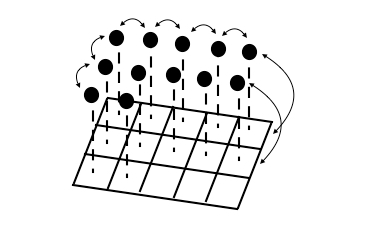
\includegraphics[width=\textwidth]{mrf_image_example}
		\caption{The idea of MRF on images the arrows indicate relations}
  \end{minipage}
  \begin{minipage}[b]{0.45\textwidth}
    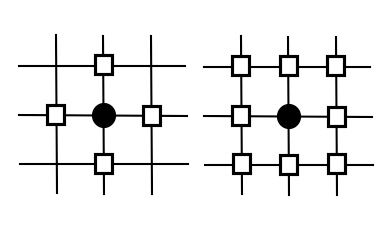
\includegraphics[width=\textwidth]{mrf_grid_neighborhood}
		\caption{4-Neighborhood ($c=1$), 8-Neighborhood ($c=\sqrt{2})$ (and dinamic-Neighborhood)}
  \end{minipage}
\end{figure}

\paragraph{Note:} that the neibhborhoods can also be decomposed in graph Cliques (complete subgraphs) of two. Which is useul later on (factorization + there are solvers for two variables)

\paragraph{Gibbs Random Fields (GRF):} is given by the PDF ($Z = \sum_{x^\prime} H(x^{\prime})$ is called a partition function and $H(x)$ is an energy function, i.e. a sum of potential functions.)

\begin{equation*}
	p(x) = \frac{1}{Z} e^{-H(x)}
\end{equation*}

\paragraph{Remark:}
For a given PDF $p(x)$, the choice of the energy function $H(x)$ is not unique. Consider for example

\begin{equation*}
	H(x) = - \log p(x) - \log Z
\end{equation*}

\begin{equation*}
	p(x) = \frac{1}{Z} e^{-H(x)} = \frac{1}{Z} e^{\log p(x)} e^{\log Z}  = p(x)
\end{equation*}

$\rightarrow$ we can choose $Z$ arbitarily\\

The interesting theoretical property is that GRFs and MRFs are equivalent. The proof for this is called Hammersley-Clifford Theorem.

\paragraph{Example:} Image denoising

Given: The observed noisy image $[g_{i,j}]$

Searched: Hidden variables are the ideal (noiseless) image $[f_{i,j}]$\\

Assumption 1: The ideal image is spatially smooth

\begin{equation*}
	p(f_{i,j}]) = \frac{1}{Z} e^{-H([f_{i,j}])}, \quad \text{where } H([f_{i,j}]) = \sum_{i,j} ||\nabla f_{i,j}||_2^2
\end{equation*}
$ H([f_{i,j}]) $ (sum of squared gradients, computed over a neighborhood)\\

Assumption 2: $[g_{i,j}]$ is similar to $[f_{i,j}]$, but corrupted by additive Gaussian noise

\begin{equation*}
	p([g_{i,j}] | f_{i,j}]) = \prod_{i,j} \frac{1}{\sqrt{2 \pi} G_{i,j}} \exp(- \frac{1}{2 G_{i,j}^2} \cdot \underset{\text{energy function $H$}}{(f_{i,j} - g_{i,j})^2})
\end{equation*}

With these two functions defined, we can solve for a MAP estimate for $f$:

\begin{align*}
	\underset{\text{estimated ideal image}}{[\hat{f}_{i,j}]} &= \argmax_{[f_{i,j}]} p([f_{i,j}] | [g_{i,j}])\\
					&= \argmax_{[f_{i,j}]} p([g_{i,j}] | [f_{i,j}]) \cdot p([f_{i,j}])\\
					& \dots\\
					& \argmin_{[f_{i,j}]} \{ \sum_{i,j} ||\nabla f_{i,j}||_2^2 + \sum_{i,j} \lambda_{i,j} (f_{i,j} - g_{i,j})^2 \}
\end{align*}

\(||\Delta f_{i,j}||_2^2\): function of clique of size 2

% TODO: Max Flow / Min Cuts
